\documentclass[11pt,a4paper]{article}
\usepackage[utf8]{inputenc}
\IfFileExists{spanish.ldf}{\usepackage[spanish]{babel}}{}
\usepackage[margin=2.3cm]{geometry}
\IfFileExists{lmodern.sty}{\usepackage[T1]{fontenc}\usepackage{lmodern}}{}
\usepackage{booktabs}
\usepackage{tabularx}
\usepackage{multicol}
\usepackage{fancyvrb}
\usepackage{graphicx}
\usepackage{amsmath}
\usepackage[hidelinks]{hyperref}
\usepackage{xcolor}

\DeclareUnicodeCharacter{2022}{\textbullet}
\DeclareUnicodeCharacter{03B5}{\ensuremath{\varepsilon}}
\DeclareUnicodeCharacter{2192}{\ensuremath{\rightarrow}}

\fvset{fontsize=\small,frame=single,framesep=2mm}
\newcommand{\code}[1]{\texttt{#1}}
\setlength{\parskip}{0.5em}
\setlength{\parindent}{0pt}

\title{Proyecto final de Lenguajes Formales\\[0.3em]
\large FIRST/FOLLOW, parsers LL(1) y SLR(1), y evaluador de SDD}
\author{Juan Camilo Estrada Rave \and Mariana Salomé Velásquez Gallego}
\date{Lenguajes Formales (SI2002-4368), Universidad EAFIT\\Noviembre de 2026}

\begin{document}
\maketitle

\section{Introducción}

El proyecto tiene tres partes, todas escritas en Python 3.14 con la librería estándar y sin librerías de parsing:

\begin{enumerate}
  \item \textbf{Ítem 1:} lectura de la gramática y cálculo de los conjuntos FIRST y FOLLOW (opción \code{--sets}).
  \item \textbf{Ítem 2:} construcción de la tabla LL(1) y de la tabla SLR(1), y los dos parsers dirigidos por tabla.
  \item \textbf{Ítem 3:} un evaluador de definiciones dirigidas por la sintaxis (SDD). El SDD se guarda como datos, y el programa construye el árbol de derivación con nuestro parser, arma el grafo de dependencias, calcula un orden topológico (o detecta un ciclo) y evalúa los atributos.
\end{enumerate}

Además, como valor agregado, hicimos un servidor web con una página que ofrece las mismas funciones desde el navegador (sección~\ref{sec:web}).

Para los tres ítems usamos una sola gramática propia, la del \emph{hechizo mágico}, que diseñamos para el SDD del ítem 3. Así el mismo ejemplo sirve de hilo conductor en todo el informe.

\section{Secciones del libro}

Seguimos a Aho, Lam, Sethi y Ullman, \emph{Compilers: Principles, Techniques, and Tools}, 2.ª edición.

\begin{center}
\begin{tabularx}{\textwidth}{@{}lX@{}}
\toprule
Sección & Qué tomamos de ella \\
\midrule
4.4.2 & Reglas de FIRST y FOLLOW. \\
4.4.3 & Construcción de la tabla LL(1) (Algoritmo 4.31) y la condición para que una gramática sea LL(1). \\
4.4.4 & Parser predictivo no recursivo con pila (Algoritmo 4.34). \\
4.5 & Análisis ascendente: movimientos shift y reduce. \\
4.6.2 & Ítems LR(0), gramática aumentada, CLOSURE, GOTO y colección canónica. \\
4.6.3 & Algoritmo de parsing LR con pila de estados (Algoritmo 4.44). \\
4.6.4 & Construcción de la tabla SLR(1) (Algoritmo 4.46). \\
5.1 & SDD, atributos sintetizados y heredados, árbol anotado. \\
5.2 & Grafo de dependencias, orden de evaluación, SDD S-atribuidos y L-atribuidos. \\
\bottomrule
\end{tabularx}
\end{center}

\section{Organización del programa y estructuras de datos}

\begin{center}
\begin{tabularx}{\textwidth}{@{}lX@{}}
\toprule
Archivo & Contenido \\
\midrule
\code{grammar.py} & Lectura de la gramática, FIRST, FOLLOW y formato de \code{--sets}. \\
\code{ll1.py} & Tabla LL(1), prueba de LL(1), parser predictivo e impresión de la tabla. \\
\code{slr.py} & Autómata LR(0), tabla SLR(1), parser LR (con traza opcional) e impresión de cajas y tabla. \\
\code{main.py} & Programa de consola de los ítems 1 y 2 (opciones \code{--sets}, \code{--tables}, \code{--trace}). \\
\code{sdd.py} & Evaluador del ítem 3. \\
\code{app.py}, \code{web/index.html} & Servidor web y página. \\
\code{test\_*.py} & 55 pruebas unitarias. \\
\code{ejemplos/} & Entradas de los ejemplos y los SDD en JSON. \\
\bottomrule
\end{tabularx}
\end{center}

\subsection*{Estructuras de datos}

\begin{itemize}
  \item \textbf{Gramática:} un diccionario \code{no terminal -> lista de alternativas}, donde cada alternativa es una lista de símbolos. Por ejemplo, \code{H -> EH e} se guarda como \code{\{"H": [["E","H"], []]\}}. La lista vacía representa $\varepsilon$: recorrerla no hace nada, que es justo lo que significa $\varepsilon$. Dentro de los conjuntos FIRST y FOLLOW, $\varepsilon$ se escribe \code{e}.
  \item \textbf{FIRST y FOLLOW:} diccionarios \code{no terminal -> set}. Se calculan por vueltas (\code{while cambio}) hasta que ningún conjunto crece.
  \item \textbf{Tabla LL(1):} diccionario con llave \code{(no terminal, terminal)} y valor la \emph{lista} de alternativas de esa casilla. Es una lista para poder detectar conflictos: la gramática es LL(1) si ninguna casilla tiene más de una alternativa.
  \item \textbf{Pilas:} listas de Python, donde el final de la lista es el tope. La del parser LL(1) empieza como \code{["\$", "S"]}; la del parser LR guarda números de estado.
  \item \textbf{Ítem LR(0):} tupla \code{(número de producción, posición del punto)}. Las producciones se numeran en una lista y la 0 es \code{S' -> S}.
  \item \textbf{Estado LR(0):} \code{frozenset} de ítems, para poder compararlo con los demás y usarlo como llave.
  \item \textbf{Tablas ACTION y GOTO:} diccionarios con llave \code{(estado, símbolo)}. Una acción es \code{("s", j)}, \code{("r", p)} o \code{("acc",)}. Si una casilla recibe dos acciones distintas, se anota un conflicto.
  \item \textbf{Árbol de derivación:} objetos \code{Nodo} con símbolo, número de producción, lista de hijos y un diccionario de atributos. Los terminales nacen con su \code{lexval}.
  \item \textbf{Grafo de dependencias:} una lista de vértices (textos como \code{H2.ant}) y una lista de aristas \code{(de, a)}, más diccionarios con lo que entra y sale de cada vértice para el orden topológico.
\end{itemize}

\section{La gramática propia: el hechizo mágico}

Un hechizo es una secuencia de elementos: \code{f} (fuego), \code{a} (agua), \code{t} (tierra) y \code{v} (viento). La gramática tiene 3 no terminales, 7 producciones y un no terminal recursivo (\code{H}):

\begin{Verbatim}
S -> H
H -> E H | e
E -> f | a | t | v
\end{Verbatim}

En el formato de entrada del programa (\code{ejemplos/gramatica\_hechizo.txt}):

\begin{Verbatim}
3
S -> H
H -> EH e
E -> f a t v
\end{Verbatim}

\section{Ítem 1: FIRST y FOLLOW}

Salida de \code{python main.py --sets}:

\begin{Verbatim}
First(E) = {a, f, t, v}
First(H) = {a, f, t, v, e}
First(S) = {a, f, t, v, e}
Follow(E) = {a, f, t, v, $}
Follow(H) = {$}
Follow(S) = {$}
\end{Verbatim}

\code{H} puede derivar $\varepsilon$, y por eso \code{e} está en FIRST(H) y en FIRST(S). FOLLOW(E) contiene FIRST(H) sin \code{e}, porque en \code{H -> E H} lo que sigue a \code{E} es \code{H}; y como \code{H} puede desaparecer, también recibe FOLLOW(H) = \{\$\}.

\section{Ítem 2: tablas y parsers}

Todas las tablas de esta sección salen de \code{python main.py --tables}.

\subsection{Tabla LL(1)}

\begin{Verbatim}
        | a       | f       | t       | v       | $
S       | S -> H  | S -> H  | S -> H  | S -> H  | S -> H
H       | H -> EH | H -> EH | H -> EH | H -> EH | H -> e
E       | E -> a  | E -> f  | E -> t  | E -> v  |
\end{Verbatim}

Ninguna casilla tiene dos producciones, así que la gramática es LL(1). La casilla \code{[H, \$]} recibe \code{H -> e} por la regla 2 del Algoritmo 4.31: la alternativa puede ser $\varepsilon$ y \$ está en FOLLOW(H).

\subsection{Autómata LR(0)}

Producciones numeradas: 0:~\code{S' -> S}, 1:~\code{S -> H}, 2:~\code{H -> E H}, 3:~\code{H -> e}, 4:~\code{E -> f}, 5:~\code{E -> a}, 6:~\code{E -> t}, 7:~\code{E -> v}.

\begin{multicols}{2}
\begin{Verbatim}[fontsize=\footnotesize]
Caja 0:
    S' -> • S
    S -> • H
    H -> • E H
    H -> •
    E -> • f
    E -> • a
    E -> • t
    E -> • v
Caja 1:
    H -> • E H
    H -> E • H
    H -> •
    E -> • f
    E -> • a
    E -> • t
    E -> • v
Caja 2:
    S -> H •
Caja 3:
    S' -> S •
Caja 4:
    E -> a •
Caja 5:
    E -> f •
Caja 6:
    E -> t •
Caja 7:
    E -> v •
Caja 8:
    H -> E H •
\end{Verbatim}
\columnbreak
\begin{Verbatim}[fontsize=\footnotesize]
Caja 0 --E--> Caja 1
Caja 0 --H--> Caja 2
Caja 0 --S--> Caja 3
Caja 0 --a--> Caja 4
Caja 0 --f--> Caja 5
Caja 0 --t--> Caja 6
Caja 0 --v--> Caja 7
Caja 1 --E--> Caja 1
Caja 1 --H--> Caja 8
Caja 1 --a--> Caja 4
Caja 1 --f--> Caja 5
Caja 1 --t--> Caja 6
Caja 1 --v--> Caja 7
\end{Verbatim}
\end{multicols}

La caja 1 representa un hechizo a mitad de camino (\code{H -> E • H}). Tiene una flecha con \code{E} hacia sí misma, porque después de leer un elemento puede venir otro.

\subsection{Tabla SLR(1)}

\begin{Verbatim}
Caja a    f    t    v    $    ||   E    H    S
0    s4   s5   s6   s7   r3   ||   1    2    3
1    s4   s5   s6   s7   r3   ||   1    8
2                        r1   ||
3                        acc  ||
4    r5   r5   r5   r5   r5   ||
5    r4   r4   r4   r4   r4   ||
6    r6   r6   r6   r6   r6   ||
7    r7   r7   r7   r7   r7   ||
8                        r2   ||
\end{Verbatim}

No hay conflictos, así que la gramática también es SLR(1) y el programa muestra el menú \code{T}~/~\code{B}~/~\code{Q}. Los reduce de \code{E} van en las cinco columnas porque FOLLOW(E) = \{a, f, t, v, \$\}. En las cajas 0 y 1, \code{H -> •} reduce con \$ (que es FOLLOW(H)): el hechizo se puede terminar ahí.

\subsection{Una cadena parseada paso a paso}

Salida de \code{python main.py --trace} con el parser SLR(1) y las cadenas \code{fat} y \code{fxa}:

\begin{Verbatim}
--- trace: fat ---
Pila              Entrada     Acción
0                 fat$        shift 5
0 5               at$         reduce E -> f
0 1               at$         shift 4
0 1 4             t$          reduce E -> a
0 1 1             t$          shift 6
0 1 1 6           $           reduce E -> t
0 1 1 1           $           reduce H -> e
0 1 1 1 8         $           reduce H -> E H
0 1 1 8           $           reduce H -> E H
0 1 8             $           reduce H -> E H
0 2               $           reduce S -> H
0 3               $           accept
yes
--- trace: fxa ---
Pila              Entrada     Acción
0                 fxa$        shift 5
0 5               xa$         error
no
\end{Verbatim}

Como la gramática es recursiva por la derecha, el parser apila todos los elementos y solo al llegar a \$ cierra el hechizo con \code{H -> e} y va reduciendo \code{H -> E H} de derecha a izquierda. En \code{fxa}, la casilla \code{[5, x]} está vacía y el parser responde \code{no}.

\section{Ítem 3: el SDD del hechizo}

\subsection{La idea}

Un hechizo es más poderoso cuanto más cambia de elemento. Cada elemento suma 1 punto si es distinto del anterior, y 0 si repite o si es el primero (que no tiene con qué compararse). Por ejemplo, \code{f a a t v} da $0+1+0+1+1 = 3$.

Para eso, cada elemento necesita saber cuál fue el anterior (un dato que viaja de izquierda a derecha: \textbf{heredado}), y el puntaje se va sumando desde las hojas hasta la raíz (\textbf{sintetizado}).

\subsection{Tabla de atributos}

\begin{center}
\begin{tabularx}{\textwidth}{@{}llllX@{}}
\toprule
Símbolo & Atributo & Clase & Tipo & Significado \\
\midrule
H, E & \code{ant} & heredado & carácter & Elemento anterior; \code{n} (ninguno) si no hay. \\
S, H, E & \code{pts} & sintetizado & entero $\geq 0$ & Puntos por cambios de elemento. \\
E & \code{el} & sintetizado & carácter & Elemento que \code{E} acaba de leer. \\
f, a, t, v & \code{lexval} & sintetizado & carácter & El carácter mismo. \\
\bottomrule
\end{tabularx}
\end{center}

\code{S} no tiene atributos heredados. El valor inicial \code{n} lo escribe la regla de \code{S -> H} sobre \code{H.ant}.

\subsection{Reglas semánticas}

\begin{center}
\begin{tabular}{@{}cll@{}}
\toprule
\# & Producción & Reglas semánticas \\
\midrule
1 & \code{S -> H} & \code{H.ant = n}; \code{S.pts = H.pts} \\
2 & \code{H -> E H1} & \code{E.ant = H.ant}; \code{H1.ant = E.el}; \code{H.pts = E.pts + H1.pts} \\
3 & \code{H -> e} & \code{H.pts = 0} \\
4 & \code{E -> f} & \code{E.el = f.lexval}; \code{E.pts = 1} si \code{E.ant} $\neq$ \code{n} y \code{E.ant} $\neq$ \code{E.el}, si no \code{0} \\
5 & \code{E -> a} & \code{E.el = a.lexval}; misma regla de \code{E.pts} \\
6 & \code{E -> t} & \code{E.el = t.lexval}; misma regla de \code{E.pts} \\
7 & \code{E -> v} & \code{E.el = v.lexval}; misma regla de \code{E.pts} \\
\bottomrule
\end{tabular}
\end{center}

En cada producción, cada atributo se define una sola vez y solo con atributos de esa misma producción. La regla clave es \code{H1.ant = E.el}: funciona como una carrera de relevos, donde el elemento que \code{E} acaba de leer se le pasa como ``anterior'' al resto del hechizo.

\subsection{Ejemplo a mano: \code{f a a t v}}

Estas son las tres entregas del ejemplo a mano, hechas por nosotros. En los dibujos los \code{H} se numeran desde \code{H0}; el programa los numera desde \code{H1} (el \code{H0} del dibujo es el \code{H1} del programa, y así sucesivamente).

\begin{center}
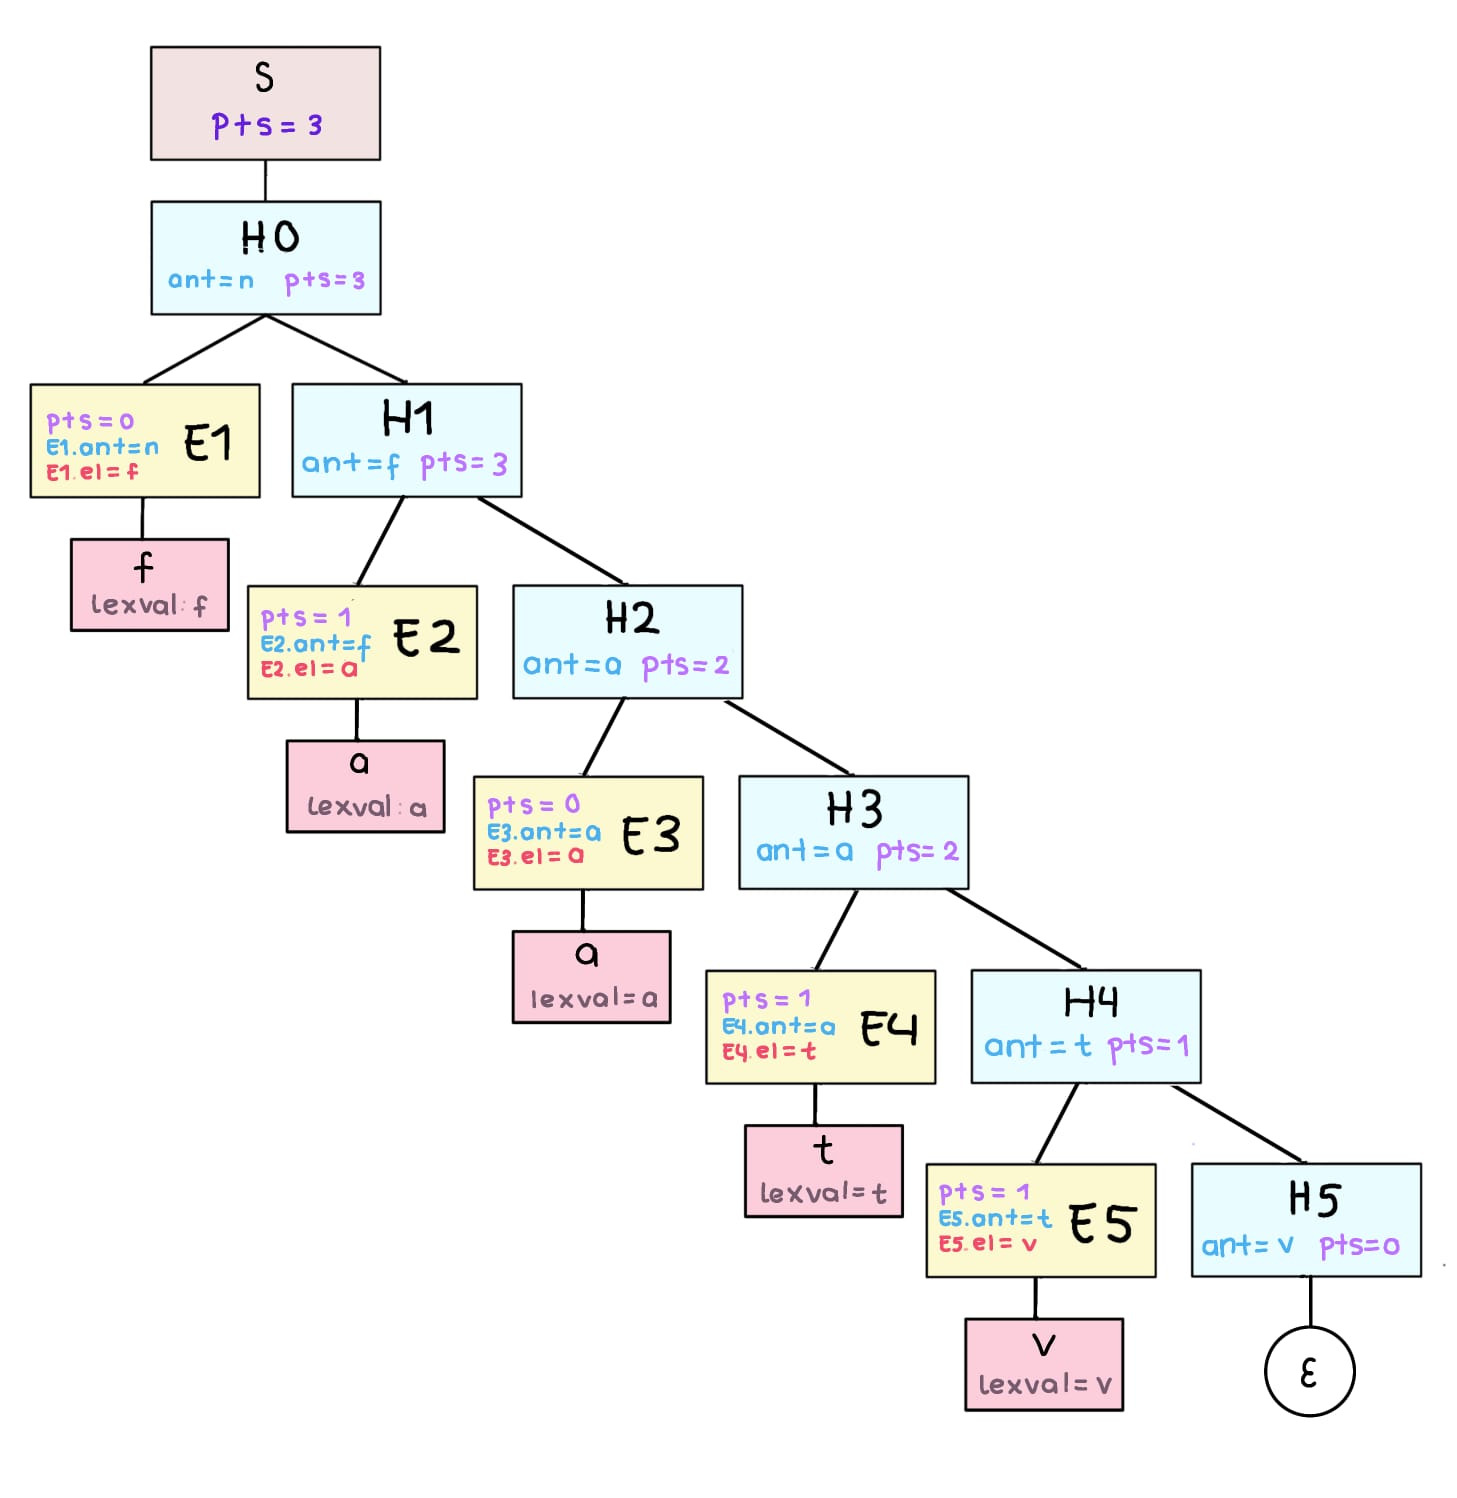
\includegraphics[width=0.6\textwidth]{figuras/arbol_faatv.png}\\[4pt]
{\small \textbf{Entrega 1 · Árbol anotado} de \code{f a a t v}: cada nodo con sus atributos (\code{ant}, \code{el}, \code{pts}, \code{lexval}). El resultado es \code{S.pts = 3}.}
\end{center}

\begin{center}
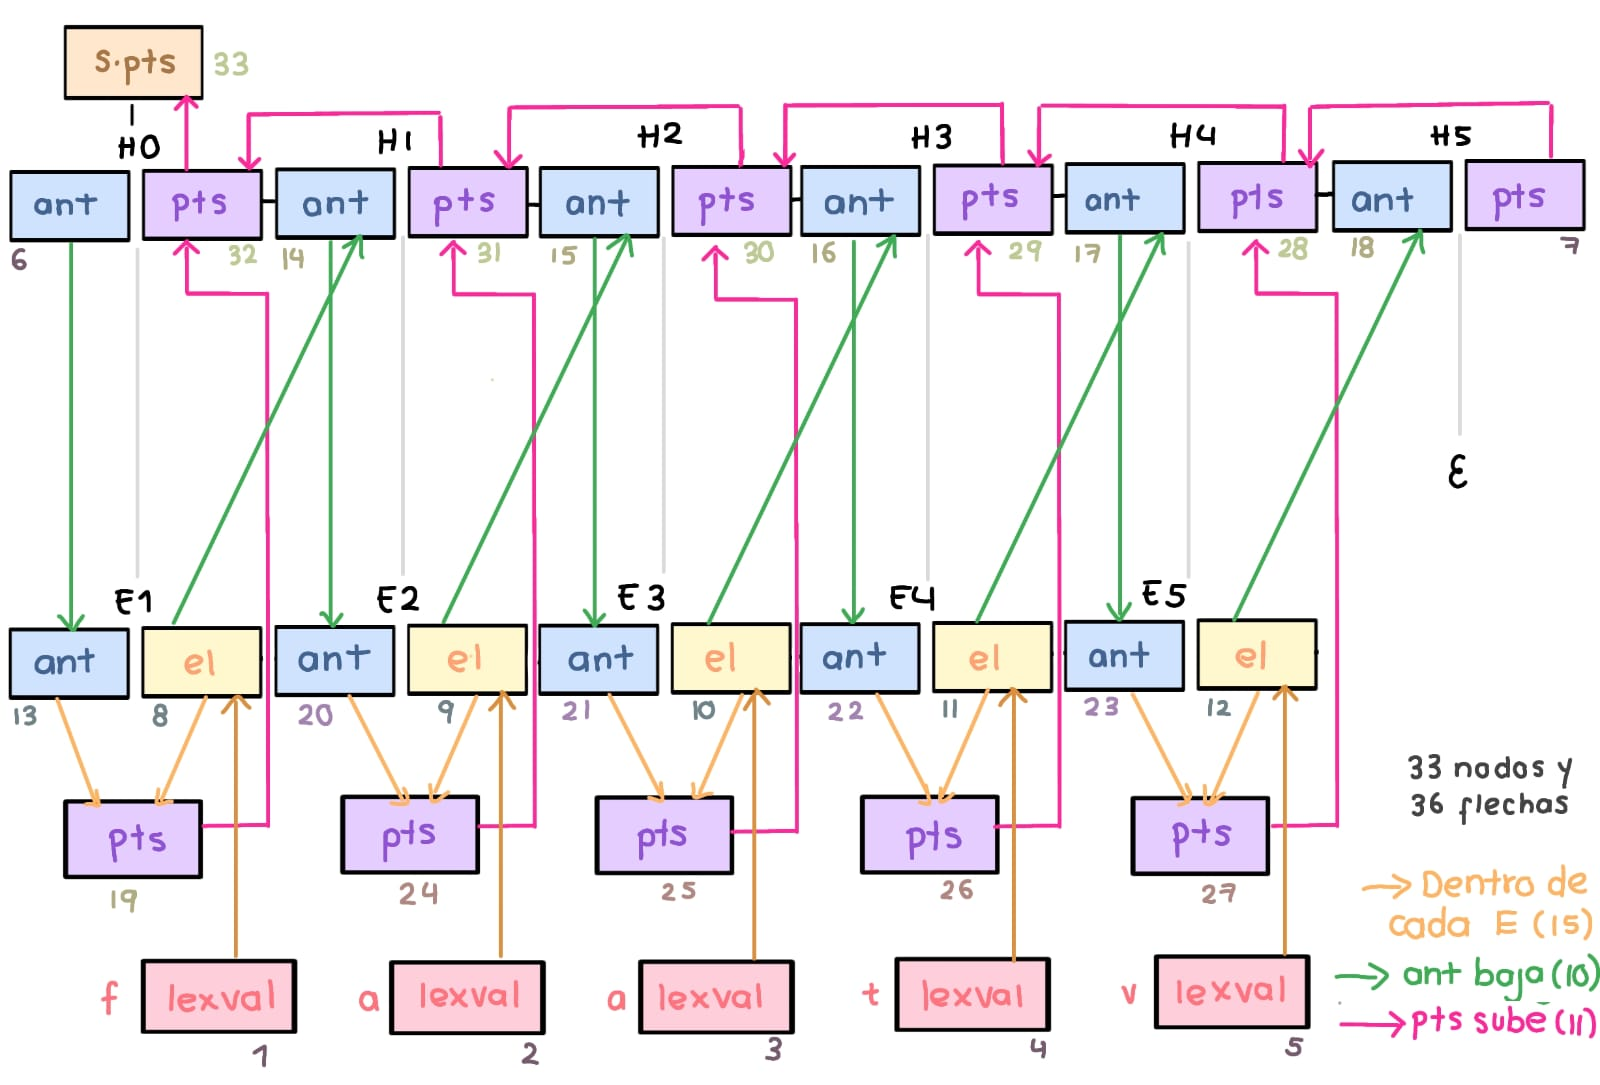
\includegraphics[width=\textwidth]{figuras/grafo_faatv.png}\\[4pt]
{\small \textbf{Entregas 2 y 3 · Grafo de dependencias y orden topológico}: 33 atributos y 36 aristas (naranja: dentro de cada \code{E}, 15; verde: \code{ant} baja, 10; rosado: \code{pts} sube, 11). El número junto a cada atributo es nuestro orden topológico, del 1 al 33: toda arista va de un número menor a uno mayor, así que es un orden de evaluación válido.}
\end{center}

El dibujo a mano coincide con lo que calcula el programa
(\code{python sdd.py ejemplos/sdd\_hechizo.json}):

\begin{multicols}{2}
\begin{Verbatim}[fontsize=\footnotesize]
S1 [pts=3]
  H1 [ant=n, pts=3]
    E1 [ant=n, el=f, pts=0]
      f1 [lexval=f]
    H2 [ant=f, pts=3]
      E2 [ant=f, el=a, pts=1]
        a1 [lexval=a]
      H3 [ant=a, pts=2]
        E3 [ant=a, el=a, pts=0]
          a2 [lexval=a]
        H4 [ant=a, pts=2]
          E4 [ant=a, el=t, pts=1]
            t1 [lexval=t]
          H5 [ant=t, pts=1]
            E5 [ant=t, el=v, pts=1]
              v1 [lexval=v]
            H6 [ant=v, pts=0]
              e
\end{Verbatim}
\columnbreak
\begin{Verbatim}[fontsize=\footnotesize]
 1. H1.ant = n     18. H5.ant = t
 2. f1.lexval = f  19. H6.ant = v
 3. a1.lexval = a  20. E2.ant = f
 4. a2.lexval = a  21. E3.ant = a
 5. t1.lexval = t  22. E4.ant = a
 6. v1.lexval = v  23. E5.ant = t
 7. H6.pts = 0     24. E2.pts = 1
 8. E1.ant = n     25. E3.pts = 0
 9. E1.el = f      26. E4.pts = 1
10. E2.el = a      27. E5.pts = 1
11. E3.el = a      28. H5.pts = 1
12. E4.el = t      29. H4.pts = 2
13. E5.el = v      30. H3.pts = 2
14. H2.ant = f     31. H2.pts = 3
15. E1.pts = 0     32. H1.pts = 3
16. H3.ant = a     33. S1.pts = 3
17. H4.ant = a
\end{Verbatim}
\end{multicols}

\textbf{Grafo de dependencias.} Tiene 33 vértices: 5 \code{lexval}, 15 de las cinco \code{E} (\code{ant}, \code{el}, \code{pts}), 12 de las seis \code{H} (\code{ant}, \code{pts}) y 1 de \code{S}. Tiene 36 aristas:

\begin{center}
\begin{tabular}{@{}lllr@{}}
\toprule
Producción & Aristas por nodo & Veces & Total \\
\midrule
\code{S -> H} & \code{H.pts} $\to$ \code{S.pts} & 1 & 1 \\
\code{H -> E H1} & \code{H.ant}$\to$\code{E.ant}, \code{E.el}$\to$\code{H1.ant}, \code{E.pts}$\to$\code{H.pts}, \code{H1.pts}$\to$\code{H.pts} & 5 & 20 \\
\code{E -> f|a|t|v} & \code{lexval}$\to$\code{E.el}, \code{E.ant}$\to$\code{E.pts}, \code{E.el}$\to$\code{E.pts} & 5 & 15 \\
\bottomrule
\end{tabular}
\end{center}

Las reglas \code{H.ant = n} y \code{H.pts = 0} son constantes y no tienen aristas de entrada. El grafo no tiene ciclos, así que existe un orden de evaluación. El orden de arriba es el que calcula el programa; uno equivalente, más fácil de hacer a mano, es por olas: primero los \code{lexval}, \code{H1.ant} y \code{H6.pts}; luego los \code{el}; luego los \code{ant}; luego los \code{E.pts}; y al final los \code{H.pts} de derecha a izquierda, terminando en \code{S.pts}.

\subsection{Clasificación}

El SDD es \textbf{L-atribuido} y \textbf{no es S-atribuido}.

\begin{itemize}
  \item \textbf{No es S-atribuido:} \code{ant} es heredado, y en un SDD S-atribuido todos los atributos son sintetizados.
  \item \textbf{Es L-atribuido:} las únicas reglas que definen un heredado son tres, y ninguna usa un hermano de la derecha: \code{H.ant = n} usa una constante; \code{E.ant = H.ant} usa un atributo del padre; y \code{H1.ant = E.el} usa un atributo de \code{E}, que está a la izquierda de \code{H1}.
\end{itemize}

\subsection{El evaluador}

\textbf{El SDD como datos.} El evaluador no sabe nada del hechizo: lee un archivo JSON con la gramática, la tabla de atributos y las reglas. Por ejemplo, la producción 2 se escribe así:

\begin{Verbatim}
"H -> E H1": ["E.ant = H.ant", "H1.ant = E.el", "H.pts = E.pts + H1.pts"]
\end{Verbatim}

Cada regla es un texto \code{Símbolo.atributo = expresión}. El programa la lee con el módulo \code{ast} de Python y revisa que solo use piezas permitidas (constantes, \code{Símbolo.atributo}, aritmética, comparaciones, \code{and}/\code{or}/\code{not}, \code{x if c else y} y unas pocas funciones como \code{max}). La expresión la evalúa nuestro propio código; nunca se usa \code{eval}. De la expresión salen solos los atributos que la regla usa, que son las aristas del grafo.

\textbf{Validación.} Antes de evaluar, el programa revisa que \code{S} no tenga heredados y que, en cada producción, se defina exactamente una vez cada sintetizado de la cabeza y cada heredado de los hijos, usando solo atributos que existen.

\textbf{Pasos para cada cadena:}
\begin{enumerate}
  \item \textbf{Árbol.} Nuestro parser SLR(1) lleva una segunda pila de nodos. Un shift crea un nodo terminal (con su \code{lexval}); un reduce toma los últimos $k$ nodos como hijos de un nodo nuevo para la cabeza. Si el parser se atasca, la respuesta es \code{no}.
  \item \textbf{Grafo de dependencias} (5.2.1). Un vértice por cada atributo de cada nodo, y para cada regla \code{X.a = f(Y.b, ...)} una arista de \code{Y.b} a \code{X.a}.
  \item \textbf{Orden topológico} (5.2.2), con el algoritmo de Kahn: se toma una y otra vez un vértice al que ya no le llegan aristas pendientes. Si quedan vértices sin tomar, hay un ciclo: el programa lo encuentra caminando hacia atrás entre los que quedaron, imprime \code{circular} y el ciclo, y se detiene.
  \item \textbf{Evaluación.} Se calculan los atributos en ese orden y se imprime el árbol anotado, el orden y el valor de \code{S.pts}.
\end{enumerate}

\subsection{Pruebas del SDD}

\begin{center}
\begin{tabular}{@{}lll@{}}
\toprule
Caso & Cadena & Resultado \\
\midrule
Ejemplo a mano & \code{faatv} & \code{S.pts = 3}, 33 vértices y 36 aristas \\
Cadena más corta & \code{f} y la vacía (\code{e}) & \code{S.pts = 0} \\
No pertenece & \code{fxa} & \code{no} \\
Anidamiento profundo & \code{fa} repetido 1500 veces & \code{S.pts = 2999} \\
Extremos & \code{ffff}, \code{fatvf} & 0 y 4 \\
SDD circular & \code{fa} & \code{circular} \\
\bottomrule
\end{tabular}
\end{center}

La versión circular (\code{ejemplos/sdd\_hechizo\_circular.json}) cambia una sola regla: \code{H1.ant = H.pts}. El hijo necesita el puntaje del padre, y el puntaje del padre necesita el del hijo. Con dos elementos el programa responde:

\begin{Verbatim}
circular
Cycle: E2.pts -> H2.pts -> H1.pts -> H2.ant -> E2.ant -> E2.pts
\end{Verbatim}

Con un solo elemento no hay ciclo, porque el último \code{H} usa la regla \code{H.pts = 0}: la circularidad depende de la cadena, como explica la sección 5.2.

\section{Servidor web}\label{sec:web}

Con \code{python app.py} se abre una página en \code{http://localhost:8000}. Está hecho solo con la librería estándar (\code{http.server}) y no cambia nada de la lógica: el servidor recibe cada pedido de la página, llama a las mismas funciones del programa de consola y devuelve el resultado en JSON. Tiene cuatro endpoints:

\begin{itemize}
  \item \code{/api/sets}: FIRST y FOLLOW.
  \item \code{/api/tables}: tabla LL(1), autómata LR(0), tabla SLR(1) y cuál de los cuatro casos es la gramática.
  \item \code{/api/parse}: \code{yes} o \code{no} con el parser elegido, y la traza del SLR(1).
  \item \code{/api/sdd}: el árbol anotado (dibujado en la página), el grafo, el orden y el valor, o \code{circular}.
\end{itemize}

El SDD se puede editar en la página, lo que muestra que el evaluador de verdad funciona con el SDD como datos.

\section{Pruebas}

Hay 55 pruebas unitarias (\code{python -m unittest test\_grammar test\_ll1 test\_slr test\_sdd}): 13 de FIRST/FOLLOW, 11 de LL(1), 14 de SLR(1) y 17 del SDD. Incluyen los tres ejemplos del enunciado, una gramática que es LL(1) pero no SLR(1), cadenas con 50 paréntesis anidados, la traza del parser, el SDD circular y SDD mal escritos que el programa debe rechazar.

\section{Problemas encontrados y cómo los resolvimos}

\begin{enumerate}
  \item \textbf{Cómo representar $\varepsilon$.} Como símbolo \code{e} se confundía con un terminal. En la gramática es una lista vacía, y así la regla de FIRST para $\varepsilon$ sale sola.
  \item \textbf{FIRST que dependen de otros todavía no calculados}, y la recursión por la izquierda (\code{S -> S+T}). Se calculan por vueltas hasta que nada cambia; una alternativa recursiva no agrega nada nuevo y el ciclo termina. No transformamos la gramática, como pide el enunciado.
  \item \textbf{Detectar que una gramática no es LL(1).} Si cada casilla guardara una sola alternativa, la segunda borraría a la primera. Cada casilla guarda una lista.
  \item \textbf{Orden al apilar una alternativa} en el parser LL(1): se apila al revés para que el primer símbolo quede en el tope.
  \item \textbf{Cuánto leer de la entrada.} \code{main.py} lee exactamente $1+n$ líneas de gramática y después las cadenas una por una, para no mezclarlas.
  \item \textbf{Ítems, CLOSURE y GOTO eran lo más abstracto.} Nos ayudó practicar shift-reduce a mano, pensar el punto como un dedo que señala lo que falta, y ver que CLOSURE y GOTO son el \code{epsilon\_closure} y el \code{move} de la conversión NFA $\to$ DFA de la entrega anterior.
  \item \textbf{Cuándo reducir.} Reducir siempre que el punto llega al final acepta cadenas malas; el reduce solo va en las columnas de FOLLOW de la cabeza.
  \item \textbf{Probar el caso ``solo LL(1)''.} Los ejemplos del enunciado no lo cubrían. Usamos \code{S -> AaAb | BbBa}, \code{A -> e}, \code{B -> e}, que tiene un conflicto reduce/reduce en SLR(1).
  \item \textbf{Representar el SDD como datos.} Escribir las reglas como funciones de Python hacía que el evaluador ``supiera'' del hechizo. Las escribimos como texto y las leemos con \code{ast}, revisando una lista blanca de operaciones en vez de usar \code{eval}, que permitiría ejecutar cualquier código.
  \item \textbf{Aristas repetidas.} La regla de \code{E.pts} usa \code{E.ant} dos veces, y el grafo salía con 41 aristas en vez de 36. Ahora cada atributo usado se cuenta una sola vez por regla.
  \item \textbf{Cadenas muy largas.} Recorrer el árbol con recursión falla con miles de nodos; el recorrido usa una pila explícita.
  \item \textbf{Un botón de la página que no hacía nada.} La función se llamaba \code{evaluate()}, el mismo nombre de una función que el navegador ya tiene (\code{document.evaluate}). La renombramos.
\end{enumerate}

\section{Uso de herramientas de inteligencia artificial}

Usamos tres herramientas, siempre con la misma forma de trabajo: \textbf{primero estudiábamos cada tema en el libro y sacábamos las ideas; después se las explicábamos a la IA y le pedíamos que nos sugiriera cómo pasarlas a código}.

\begin{itemize}
  \item \textbf{Cómo trabajamos.} Para cada algoritmo, primero lo leíamos en el libro y lo hacíamos a mano con ejemplos pequeños (FIRST y FOLLOW, tablas LL(1), cajas LR(0), tabla SLR, el árbol y el grafo del SDD). Con esas ideas decidíamos cómo representarlo (por ejemplo, $\varepsilon$ como lista vacía, o el SDD como un archivo JSON) y se lo explicábamos a la IA. La IA nos sugería cómo escribirlo en código; nosotros revisábamos esa sugerencia línea por línea, la ajustábamos y la probábamos contra nuestros resultados a mano.
  \item \textbf{Claude} (Anthropic): nos explicó los temas con analogías y ejercicios interactivos, y nos ayudó a escribir el código de los módulos, las pruebas, el README y este informe. También nos mostró funciones y módulos de Python que no conocíamos, como \code{frozenset}, \code{setdefault}, \code{ast}, \code{redirect\_stdout} y \code{http.server}.
  \item \textbf{Gemini} (Google): para traducir y resumir secciones del libro antes de leerlas.
  \item \textbf{Claude Code}: para los commits y el repositorio de GitHub.
\end{itemize}

El diseño del SDD (la idea del hechizo, los atributos, las reglas y la clasificación) lo hizo Mariana, eligiendo y justificando cada decisión en ejercicios guiados paso a paso. Los ejemplos a mano los hicimos nosotros, como pide el enunciado.

\end{document}
